
\documentclass{article}

\usepackage{times}
\usepackage{hyperref}
\usepackage{tikz}
\usepackage{bibunits}
\usepackage{natbib}
\usepackage{graphics}
\usepackage{amsmath}
\usepackage{indentfirst}
\usepackage[utf8]{inputenc}
\usepackage{graphicx}

\DeclareMathOperator{\var}{var}
\DeclareMathOperator{\cov}{cov}

\usepackage{Sweave}
\begin{document}
\Sconcordance{concordance:interimreport1.tex:interimreport1.Rnw:%
1 19 1 1 0 73 1 1 17 2 1 1 4 16 0 1 2 4 1 1 4 16 0 1 2 4 1 1 4 16 0 1 2 %
4 1 1 4 16 0 1 2 6 1 1 70 2 1 2 2 6 1 2 2 6 1 2 2 6 1 2 2 6 1 1 9 1 2 8 %
1 1 9 1 2 68 1 1 4 2 1 1 4 16 0 1 2 4 1 1 4 2 1 1 4 13 0 1 2 4 1 1 4 2 %
1 1 4 12 0 1 2 5 1 1 4 2 1 1 4 25 0 1 2 4 1 1 4 2 1 1 4 10 0 1 2 295 1}


\title{Measles risk assessment and cost interim report\\ \vspace{2 mm} {\large David T S Hayman, Tim Carpenter,\\ Jonathan C Marshall, Mick Roberts, Nigel P French}}
\author{mEpiLab and EpiCentre,\\ Infectious Diseases Research Centre,\\
Massey University,\\
Palmerston North 4442,\\
New Zealand\\
\href{mailto: D.T.S.Hayman@massey.ac.nz}{D.T.S.Hayman@massey.ac.nz}}  %\texttt formats the text to a typewriter style font
\date{\today}  %\today is replaced with the current date
\maketitle

\section{Abstract}

Summary of findings

\section{Background}

As a member of the World Health Organization (WHO) Western Pacific Region, New Zealand is committted to work towards measles elimination, defined as the interruption of endemic (domestic) measles virus transmission, as achieved in the Americas in 2002. The Western Pacific Region is expected to be the second WHO region to  achieve measles elimination and it was announced that in March 2014 that Australia, Macao, Mongolia and the Republic of Korea have achieved this.

The last widespread measles outbreaks in New Zealand occurred in 1991 and in 1997. Since then, smaller but significant outbreaks have occurred in 2009 (mainly in Canterbury) and in 2011/2012 (mainly in Auckland region) and another significant outbreak is currently going on in the Auckland and Waikato regions. The outbreak in 2011-2012 lasted for more than 12 months and the current 2013/2014 outbreak started at the end of December 2013 (as on \date{\today}). In 2013, prior to the 2013/2014 outbreak, New Zealand was advised by the Western Pacific Regional Verification Commission for Measles Elimination (RVC) it can request verification of non-endemic status three years after the last case of the 2011-12 outbreak in June 2012.

Previous analyses, including two of measles in New Zealand by Prof. Roberts (INSERT REFS), have estimated that the interruption of measles virus transmission can be achieved by herd immunity when approximately 95 percent of the population is homogeneously immune to measles. Thus, while New Zealand immunisation activities have led to measles outbreaks becoming less frequent, with decreasing numbers of cases, as described above, outbreaks still occur. Current overall population immunity estimates suggest that approximately 85 to 90 percent of the population is immune to measles, thus the reasons for the ongoing outbreaks are perhaps likely due to overall population immunity being less than 95 percent and there being pockets of susceptible, non-immune population remaining. Since 2009, all the outbreaks in New Zealand were linked to infections acquired (imported) from overseas, though previous work suggests these outbreaks still largely affect school-aged children and children under two years of age. Under two year olds are thought be be consistently among the most affected age groups because the first of two doses of measles, mumps and rubella vaccine (MMR) is not due until fifteen months.

\section{Risk analysis review}

A measles risk assessment has been started by the Ministry of Health to better assess current and future population immunity and high risk groups. Given the current measles outbreak, measles control is a priority for the Ministry and resources are available to control this outbreak and decrease the risk of future outbreaks.
\begin{itemize}
\item In this section we review the confidential report to the Western Pacific Regional Verification Commission for Measles Elimination risk assessment provided by the Ministry, titled \emph {Progress Towards Measles Elimination in New Zealand - Final}.
\end{itemize}

Overall, we thought the review was very thorough. The report included substantial background information on measles immunisation in New Zealand (\emph{section 1.3}), the epidemiology of measles in New Zealand (\emph{section 2}), the quality of epidemiological surveillance and laboratory testing for measles (\emph{section 3}), and the levels of population immunity against the virus (\emph{section 4}). Additional details are included for many aspects of measles epidemiology and control, not least regarding the recent MMR coverage rates by birth cohort in New Zealand (\emph{section 4.2}) and the sustainability of the national immunisation programme (\emph{section 5}).

Within the report there are many tables and figures which given substantial detail on the measles situation in New Zealand. Overall these were of high quality, reporting both absolute measles case numbers and rates per 100,000 population in New Zealand.

Specific epidemiological details were provided for the 2011/2012 outbreak including \emph{Figure 4}, the number and classification of measles notifications in New Zealand by month, 2011 and 2012, with additional breakdown by age group, 2011 and 2012 (\emph{Figure 5}) and per 100,000 population (e.g. \emph{Figures 6-8}). Similar presentation of the case data are provided for ethnicity (e.g. \emph{Figures 9-10}) and New Zealand Index of Deprivation (NZDep) (e.g. \emph{Figures 11-13}). Three figures,\emph{Figures 12, 13,} and \emph{28}, show that there is spatial clustering of cases.

The report concludes that New Zealand's surveillance system has been performing well and that the Ministry is confident that measles has not been circulating since June 2012 and has not become endemic in NZ. We agree with the statement that measles is not endemic and provide some preliminary analyses on the outbreaks since endemic measles 'elimination' (see section X) that gives information regarding the likelihood of this occuring.

We agree with the report's conclusions that testing for measles is performed appropriately within the required timeframe, but clearly improving inter-laboratory communication and collaboration and timeliness of the testing and reporting is necessary for rapid responses to measles introductions.

Vaccination coverage presented in the report and to ourselves confirms that immunisation levels are approaching 94\% for MMR dose one (birth cohorts 2009 and 2010) and 89\% for MMR dose two (birth cohorts 2006 and 2007). However, only Asian and Pacific ethnicities have consistently had MMR dose one coverage approching or over 95\% levels for cohorts from 2007 onwards, and thus we agree with the report's conclusions that timeliness and coverage of vaccination need improving. This is particularly in light of our modeling results (section X).

The analyses we thought could further inform the understanding of risk from measles infection were:
\begin{itemize}
\item Multivariate modelling to account for confounding within the univariate analyses.
\item Inclusion of multivariate model results with local level immunity data to develop a risk map for NZ. 
\item Analyses of changing risk factors through time during outbreaks.
\item Modelling transmission chains in the population to understand effective reproduction number.
\item Development of risk maps to understand measles importation.
\end{itemize}

\section{Additional risk analyses}

In this section we provide a brief description of the work we are performing that we believe will help inform the Ministry of Health regarding the understanding of risk from measles. These analyses are intended to build on the excellent analyses already included in the \emph {Progress Towards Measles Elimination in New Zealand - Final} report reviewed above.

We received the raw case data from The Institute of Environmental Science and Research Ltd (ESR) EpiSurv on 27 June 2014. Initial analyses of those data suggest that we require denominator data to perform multivariate analyses. Specifically for the multivariate analyses we wish to perform we require \emph{Age * Prioritized Ethnicity * NZDep} data for New Zealand to see if the interactions among case covariates give us any additional information on risk from the univariate analyses already performed in the report reviewed above.

These data are currently unavailable in the form we require and after contacting ESR and NZ Statistics we and NZ statistics have contacted the University of Otago to see if we can obtain these denominator data. Additional data we believe would enable us and the Ministry to understand measles risk better is fine scale (lower than DHB) immunization coverage data.

We have reviewed the information on measles importation and the origins of the introductions of measles into New Zealand. To help better understand the risk of measles importation, with a particular goal of enabling the Ministry to better inform travellers, we sought to understand better the risk of measles importation. For our initial analyses, we used the arrivals data from \href{http://www.immigration.govt.nz/}{www.immigration.govt.nz} as an estimate of human movement to and from New Zealand. We collated country population size, measles incidence and measles vaccination cover from the WHO \href{http://www.who.int/research/en/}{www.who.int/research/en/}.


\begin{table}
\caption{Immigration to New Zealand (2012)}
%latex.default(immigration, file = "", table.env = FALSE, rowname = NULL)%
\begin{center}
\begin{tabular}{lr}
\hline\hline
\multicolumn{1}{c}{id}&\multicolumn{1}{c}{immigration}\tabularnewline
\hline
Australia&$809775$\tabularnewline
United Kingdom&$306177$\tabularnewline
China&$256036$\tabularnewline
United States&$194438$\tabularnewline
Japan&$ 86676$\tabularnewline
Germany&$ 83608$\tabularnewline
Korea, Republic of&$ 73459$\tabularnewline
France&$ 71448$\tabularnewline
India&$ 69038$\tabularnewline
Canada&$ 54981$\tabularnewline
\hline
\end{tabular}\end{center}\end{table}

\begin{table}
\caption{Lowest national measles vaccine cover (2012)}
%latex.default(vaccinecover, file = "", table.env = FALSE, rowname = NULL)%
\begin{center}
\begin{tabular}{lr}
\hline\hline
\multicolumn{1}{c}{id}&\multicolumn{1}{c}{cover}\tabularnewline
\hline
Equatorial Guinea&$34$\tabularnewline
Somalia&$49$\tabularnewline
Lesotho&$60$\tabularnewline
Central African Republic&$65$\tabularnewline
Papua New Guinea&$67$\tabularnewline
Chad&$69$\tabularnewline
Haiti&$69$\tabularnewline
South Sudan&$70$\tabularnewline
Gabon&$71$\tabularnewline
Yemen&$71$\tabularnewline
\hline
\end{tabular}\end{center}\end{table}

\begin{table}
\caption{Measles Incidence per million (2012)}
%latex.default(incidence, file = "", table.env = FALSE, rowname = NULL)%
\begin{center}
\begin{tabular}{lr}
\hline\hline
\multicolumn{1}{c}{id}&\multicolumn{1}{c}{incidence}\tabularnewline
\hline
Equatorial Guinea&$1617$\tabularnewline
Nauru&$1100$\tabularnewline
Democratic Republic of the Congo&$1096$\tabularnewline
Somalia&$ 979$\tabularnewline
Djibouti&$ 824$\tabularnewline
Sudan&$ 786$\tabularnewline
Burkina Faso&$ 447$\tabularnewline
Romania&$ 342$\tabularnewline
Ukraine&$ 280$\tabularnewline
Sudan&$ 229$\tabularnewline
\hline
\end{tabular}\end{center}\end{table}

\begin{table}
\caption{Risk of measles importation to New Zealand in 2012}
%latex.default(risk, file = "", table.env = FALSE, rowname = NULL)%
\begin{center}
\begin{tabular}{lr}
\hline\hline
\multicolumn{1}{c}{id}&\multicolumn{1}{c}{risk}\tabularnewline
\hline
United Kingdom&$10202161$\tabularnewline
Australia&$ 6991116$\tabularnewline
Malaysia&$ 3226580$\tabularnewline
Thailand&$ 1576414$\tabularnewline
China&$ 1138900$\tabularnewline
India&$ 1039356$\tabularnewline
Indonesia&$  984022$\tabularnewline
Ukraine&$  664315$\tabularnewline
Ireland&$  585413$\tabularnewline
Romania&$  490731$\tabularnewline
\hline
\end{tabular}\end{center}\end{table}

The preliminary analyses of 2012 data suggest immigration (whether for work, pleasure, etc.) is dominated by Australia, United Kingdom, China, and the United States, as shown in Table 1. However, vaccination coverage is lowest and measles incidence highest in less developed nations (Tables 2 and 3). Though the interactions between these different risk factors are unknown, simple products of measles incidence in 2012 and immigration numbers in 2012 suggest that though immigration is lower from some Asian countries, travel from (and thus we presume to) some countries also poses a risk. These data are shown in Table 4. The data for all the variables for each nation state and territories for 2012 are plotted in Figure 1 and the risk map for measles incidence and immigration in Figure 2.


\begin{figure}[h!]
\begin{center}
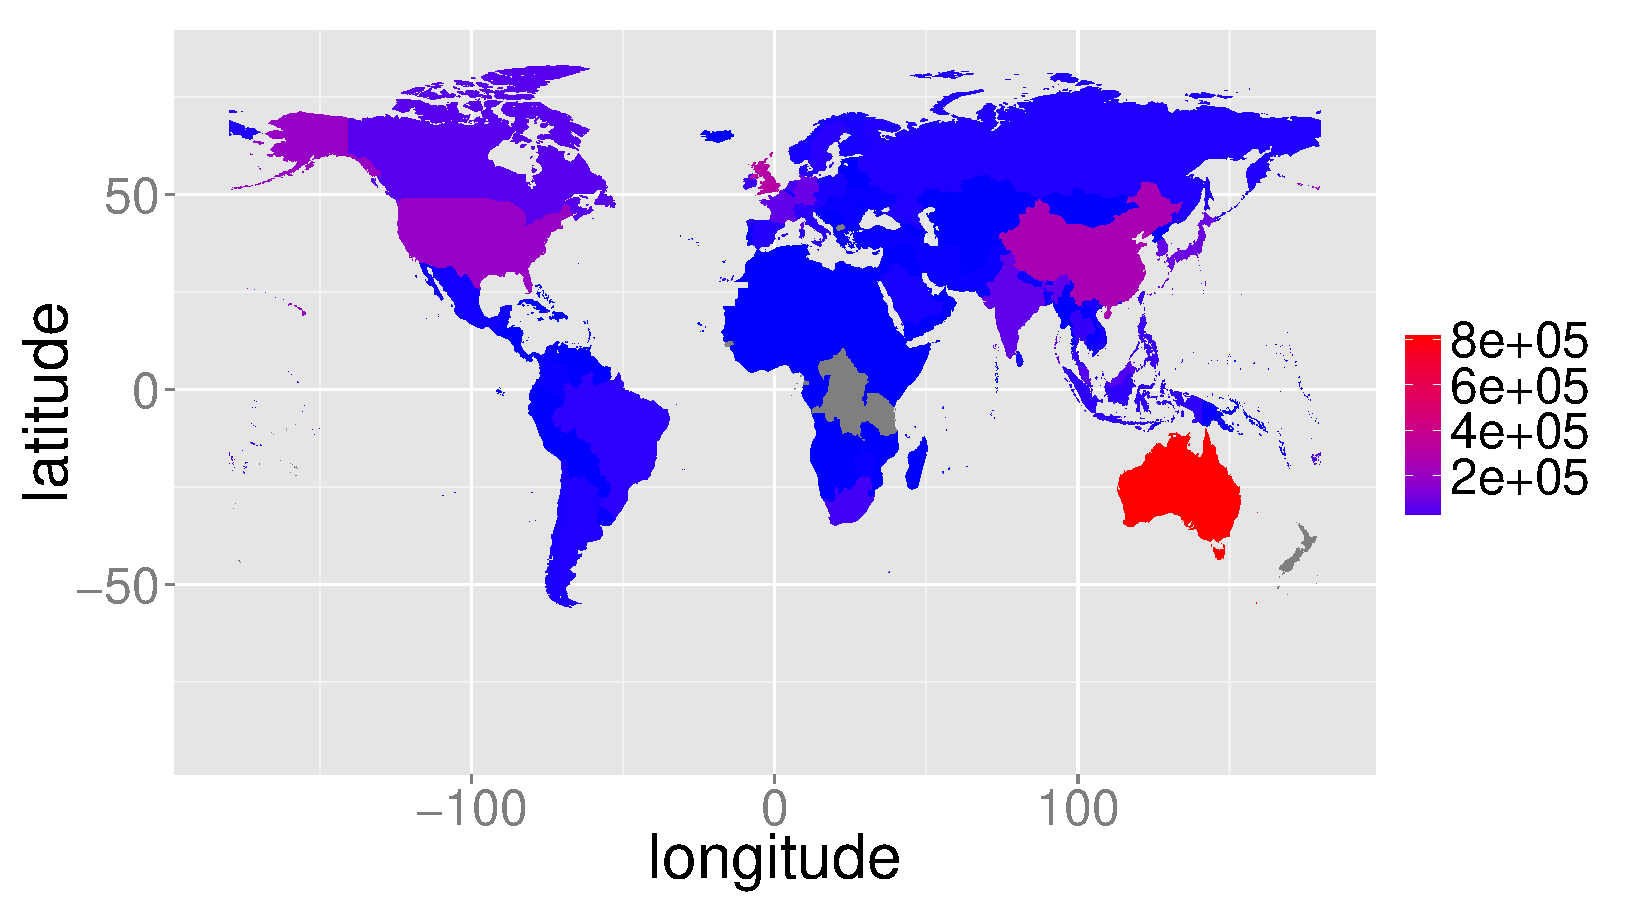
\includegraphics{interimreport1-007}
\end{center}
\caption{Immigration to New Zealand 2012}
\end{figure}

\begin{figure}[h!]
\begin{center}
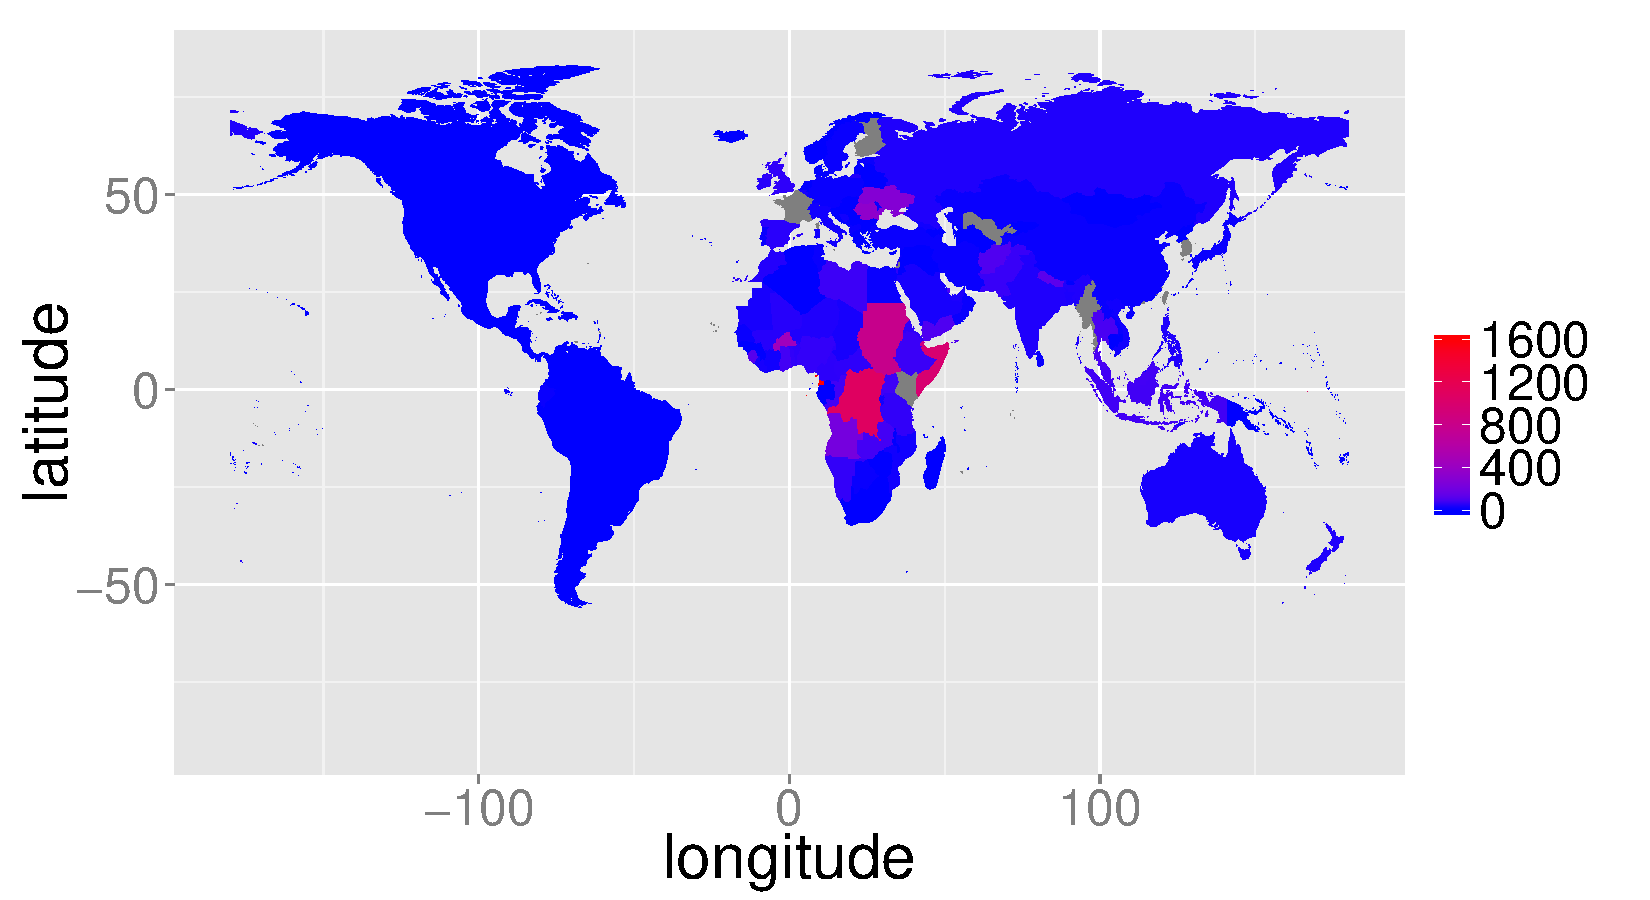
\includegraphics{interimreport1-008}
\end{center}
\caption{Measles incidence per million 2012}
\end{figure}

\begin{figure}[h!]
\begin{center}
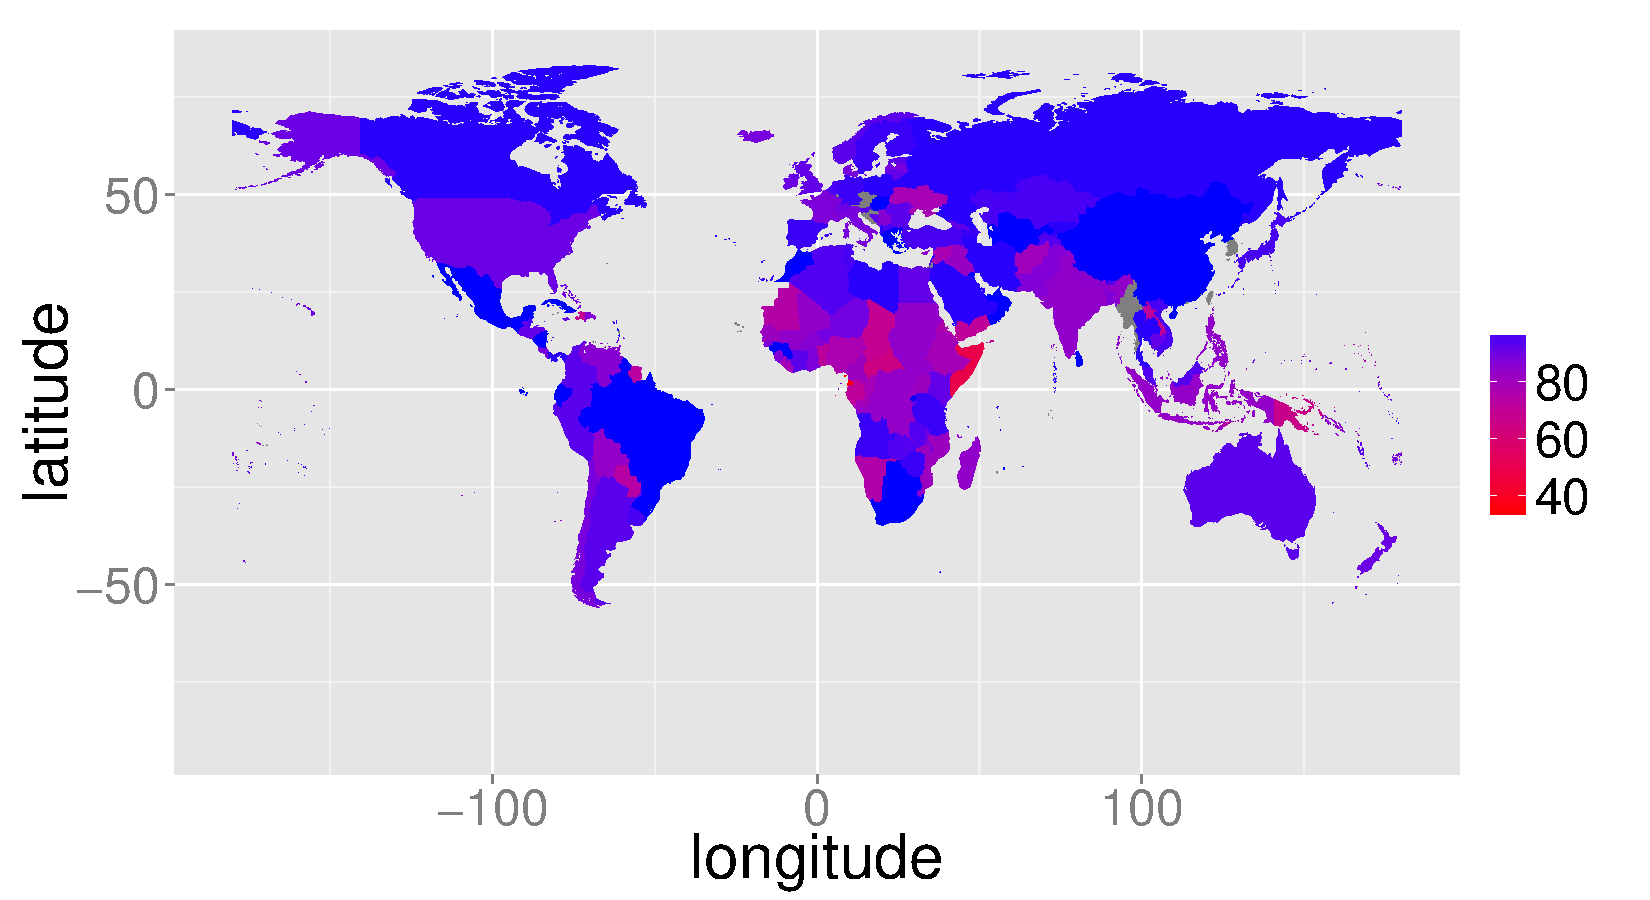
\includegraphics{interimreport1-009}
\end{center}
\caption{Measles vaccination cover (\%) 2012 }
\end{figure}

\begin{figure}[h!]
\begin{center}
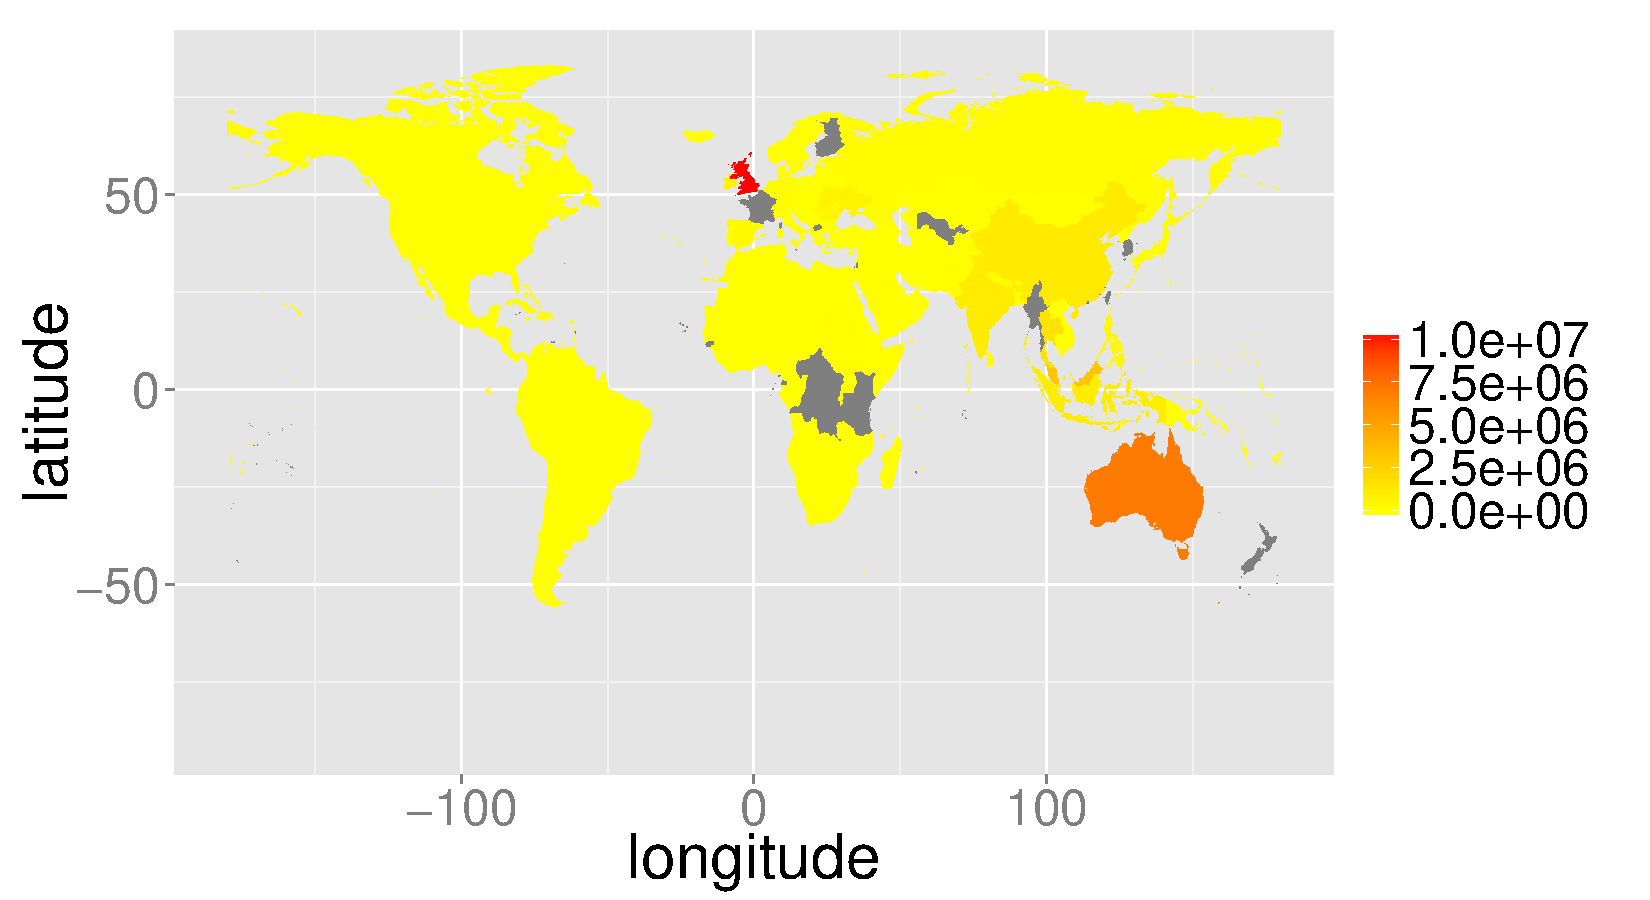
\includegraphics{interimreport1-010}
\end{center}
\caption{Risk map from measles incidence and immigration rates}
\end{figure}

\section{Future risk analyses}
We received ESR EpiSurv measles case data on the 27 June 2014. The following are analyses are still in progress and aim to include them in later reports:
\begin{itemize}
\item Multivariate regression analyses to look for interactions between risk factors that may confound the univariate analyses.
\item Update of the importation risk analyses using more than the 2012 data.
\end{itemize}
The data gaps that we have that will hinder us in completing all the analyses are:
\begin{itemize}
\item A lack of meshblock level immunisation coverage data to allow targeted immunisation and understanding of risk at a fine scale level. We understand the National Immunisation Register (NIR) allows tracking of the vaccination status of children and this is very useful, but inclusion of these data at lower (e.g. \emph{meshblock}) level would allow better understanding of risk and resource allocation.
\item A lack of data at any level that combines NZDep with age, prioritized ethnicity, and other variables, that allow better use of data collected by the Ministry, ESR, and NZ statistics for multivariate analyses.
\end{itemize}

\section{Cost analyses}

In this section we provide an analysis of the costs involved with this current measles outbreak.

... [TEXT HERE] ...

\section{Future cost-benefit analyses}
Using the results above we aim to:
\begin{itemize}
\item Estimate the costs for targeted vaccination, based either on the univariate analyses presented to date and in the \emph {Progress Towards Measles Elimination in New Zealand - Final} report or adjusted if any additional risk groups are identified if the multivariate analyses can be performed once appropriate denominator data are obtained.
\end{itemize}

\section{Modeling measles epidemics}

A previously-published model of the dynamics of measles infections
in New Zealand has been used to evaluate the vaccination strategy in New Zealand of
MMR1 at 15 months and MMR2 before 5 years. The results show that
achieving coverage of >90\% at both vaccination opportunities is
necessary if future epidemics of measles are to be prevented. [AND LIKELY MORE?!]

The original mathematical model for the dynamics of measles in New Zealand
was prepared in 1996 (Tobias & Roberts 1998). It successfully predicted the
1997 epidemic, which was curtailed by a mass vaccination campaign (Mansoor
et al 1998; Roberts & Tobias 2000). A subsequent extension of this work in
1998 showed that the then current schedule of MMR1 at 15 months and MMR2
at 11 years was insufficient to prevent further epidemics. The schedule was
changed in 2000 with MMR2 now being administered before 5 years (Anon.
2002a).

A variety of similar models for measles vaccination strategies have been developed
by other authors for various regions (Agur et al 1993; Babad et al 1995;
Edmunds et al 2000; Gay et al 1998; Wallinga et al 2001). These have invariably
been based on sets of nonlinear differential equations, and the conclusions
reached have been similar. The differences in the models have been in the details
of the representation of the infectious period, and in the ways in which
the age and contact structures of the population have been specified.

The model developed by Roberts & Tobias (2000) supported the change in the
immunisation schedule that took effect in January 2001, at which time MMR2
was changed from delivery at 11 years to delivery before the age of five. These
results were in line with those obtained by other authors, for example: Babad
et al (1995) advocated a two-dose schedule for England and Wales, with the
second vaccination given at age four; and Gay et al (1998) recommended a
second vaccination at either 18 months or five years, to complement the first
vaccination at 12 months in Canada. In addition, Agur et al (1993) found that
vaccinating 85\% of susceptible children aged one to seven years at five-yearly
intervals would prevent epidemics in Israel. These authors all agree that two
vaccinations at no less than five years apart are necessary to prevent measles
epidemics.
A different approach was taken by Wallinga et al (2001). These authors took
existing policies in eight European countries and estimated the coverage rates
required to reduce Rv below one. They found that results depended on the
age at delivery, but no strategy succeeded if coverage rates were below approximately
87\%. Our results presented in Table 1 are similar where coverage is
assumed to be the same at MMR1 and MMR2. The results also show the absolute
necessity of maintaining high coverage rates in order to prevent future
epidemics. It is difficult to estimate the proportion of the school-age population
that have been effectively immunised, but this is continuously being
diluted by children who are not immunised. Wallinga et al (2000) noted that
in Italy only MMR1 was offered at 18 months with no second vaccination opportunity,
and that under most plausible assumptions for contact rates even
100\% coverage would be insufficient to prevent epidemics.
Our final conclusion must depend on how much faith is placed in the model.
The results are consistent with those of other authors, and from Table 1 it
could be deduced that 85\% coverage at MMR1 and MMR2 could be sufficient
to prevent future measles epidemics. However, a study by Glass et al (2004)
in the Netherlands showed that high overall levels of measles vaccination can
obscure pockets of poor coverage, resulting in localised regions with increased
risk of infection. Our results indicate that overall targets or 90\% or more will
need to be achieved to prevent future epidemics in New Zealand.

The quantity that determines whether an epidemic will occur is the basic
reproduction number of the infection, R0. This is defined as the expected
number of secondary infections that would arise from a single primary infection
introduced into a fully susceptible population (Anderson & May 1991;
Diekmann & Heesterbeek 2000). Clearly if R0 > 1 an epidemic will occur following
an introduction of infection. The best estimate we had for measles in
New Zealand was R0 = 12.8, the change in the birth rate (56780 p.a. in 2004,
www.stats.govt.nz) could have reduced this slightly to R0 = 12.5 (see results
section). Recall that R0 is calculated in the absence of control measures. We
are interested in two related quantities:

The basic reproduction number of the infection under vaccination, Rv,
is the expected number of secondary infections that would arise from a
single primary infection introduced into a vaccinated population at equilibrium.
This is a robust indicator of the performance of a vaccination
schedule. If Rv < 1 epidemics are prevented.

The case reproduction number of the infection at time t, Rt, is the
expected number of secondary infections that arise from a single infection
at a particular time. This depends on the number in the population who
are susceptible, either through prior infection or vaccination.

The dynamics of the process may be summarised as follows. Assume that
the population has Rt < 1 for measles. As the number of susceptibles in the
population increases, through children that miss their scheduled immunisations,
then Rt increases. An epidemic occurs when Rt has increased above
one. During the epidemic the number of susceptibles and hence Rt decreases.


Calculated values of Rv for the various coverage levels of MMR1 and MMR2
that were considered are presented in Table 1.

\begin{figure}
     \centering
     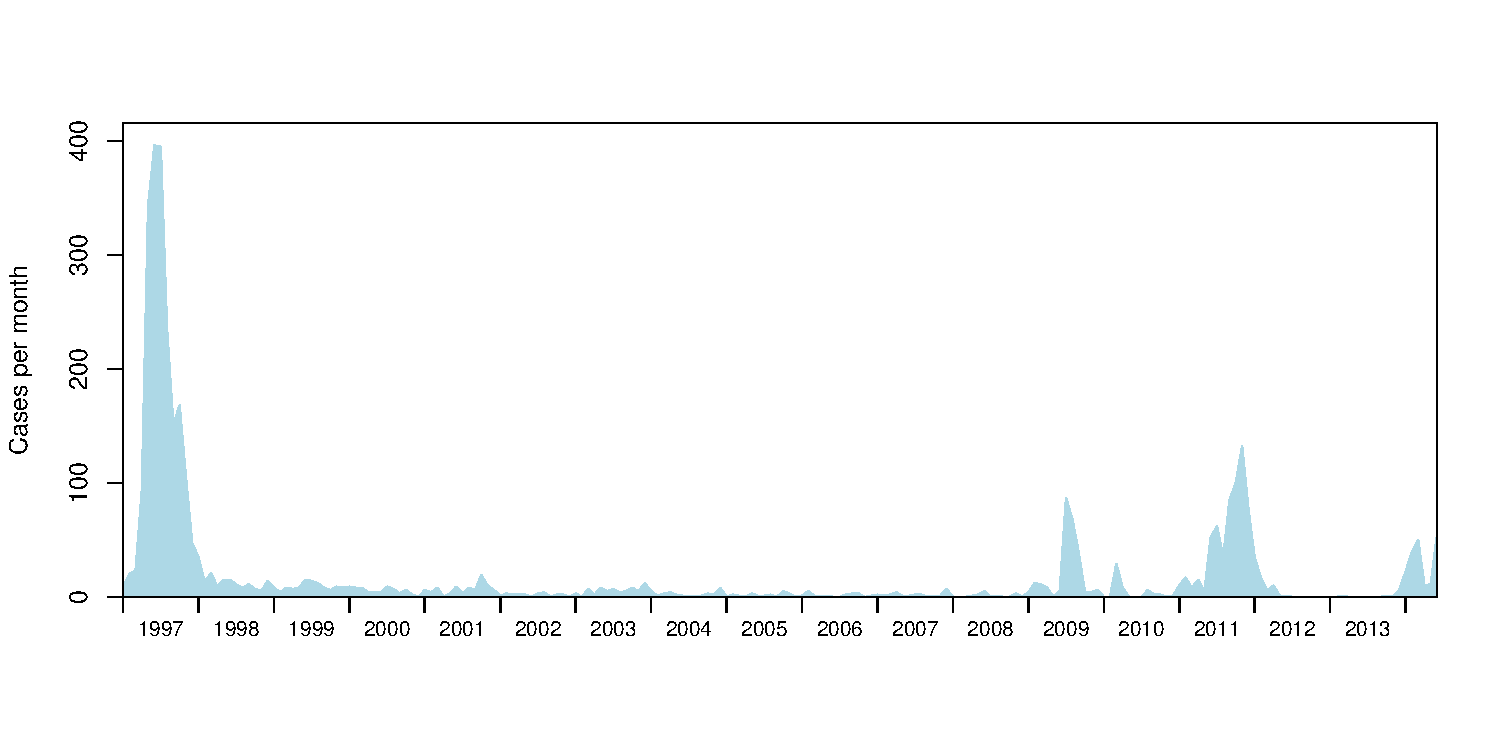
\includegraphics[width=0.8\textwidth]{incidence_1997_2014.pdf}
     \caption{Measles incidence from 1997 to 2014}
     %\label{fig:test image}
\end{figure}

\begin{figure}
     \centering
     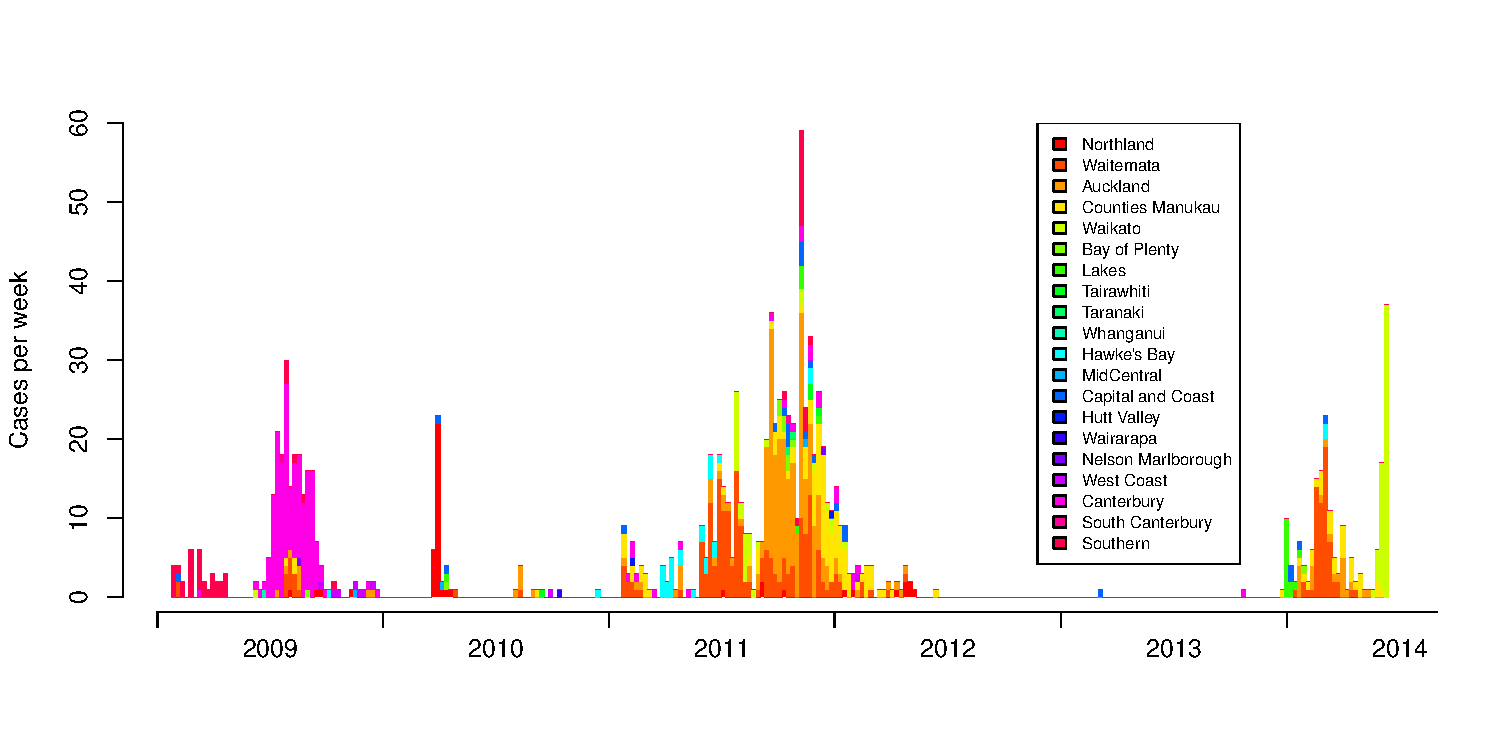
\includegraphics[width=0.8\textwidth]{cases_by_dhb_2009_2014.pdf}
     \caption{Measles cases by DHB from 2009 to 2014}
\end{figure}

\begin{figure}
     \centering
     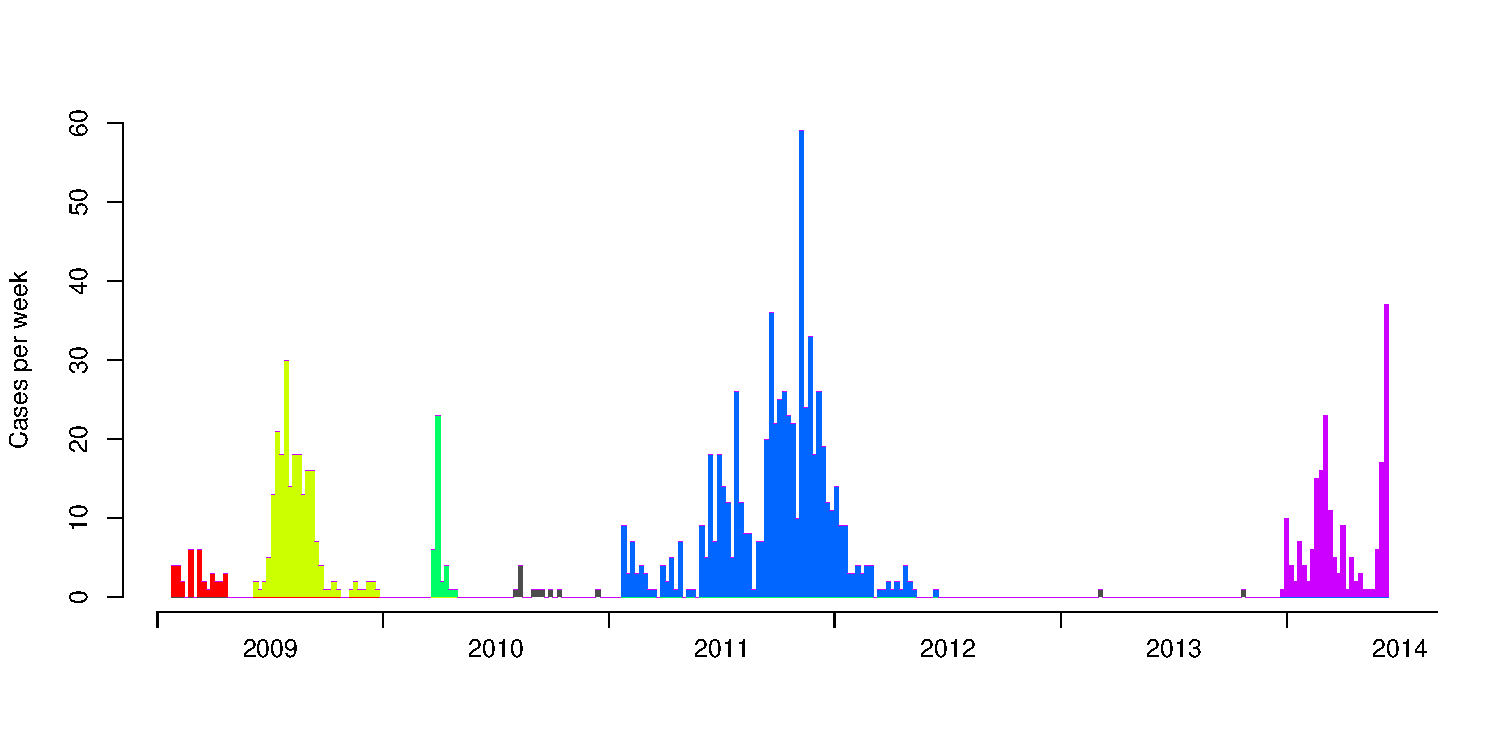
\includegraphics[width=0.8\textwidth]{outbreaks_for_R0.pdf}
     \caption{Measles data classified as outbreaks for R0 estimation}
     \label{fig:outbreaks}
\end{figure}

\begin{figure}
     \centering
     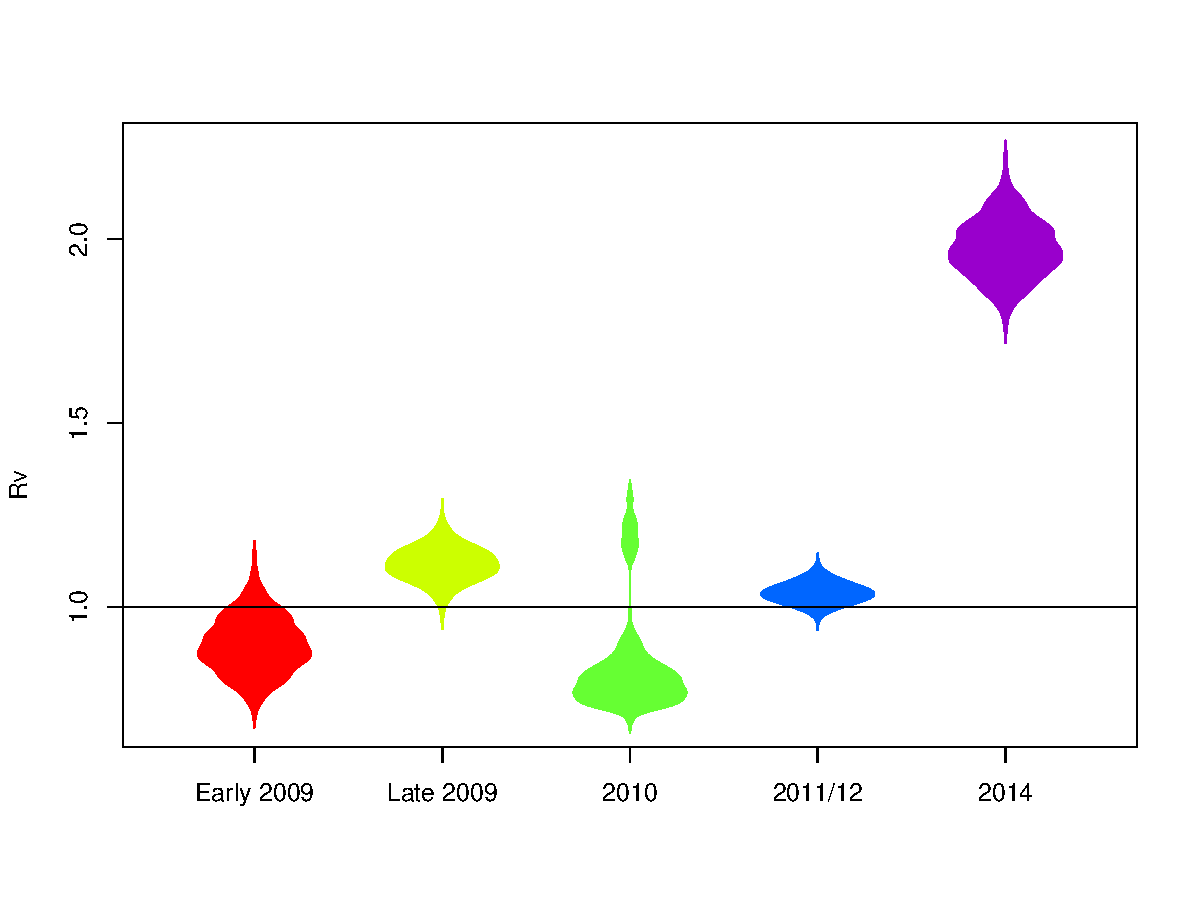
\includegraphics[width=0.8\textwidth]{averageR0.pdf}
     \caption{Estimates of R0 for the outbreaks each year, as classified in Figure~\ref{fig:outbreaks} (page~\pageref{fig:outbreaks})}
\end{figure}

...The report also concludes that increased immunisation uptake during the 2011-2012 outbreak, especially in the Auckland region, likely contributed to minimise the number of cases. [COMMENT? Unsure, though don't want to be dismissive].
....

\section{Future analyses}

\section{Future cost-benefit analyses}
Using the results above we aim to:
\begin{itemize}
\item Update previous ODE models of measles outbreak risk in the overall population according the differing vaccine coverage scenarios.
\item Model measles outbreaks with differing scenarios of measles importation into various population groups based on current introduction rates.
\end{itemize}

\section{Acknowledgments}
The authors wish to thank Tomasz Kiedrzynski, Lisa Oakley and Nic Aagaard from the Ministry of Health, Ruth Pirie and colleagues from ESR for help in obtaining the appropriate materials for analyses.

\begin{thebibliography}{}

\bibitem[Gelman et al.(1996)Gelman, Roberts, and Gilks]{grg}
Gelman, A., G.~O. Roberts, and W.~R. Gilks (1996).
\newblock Efficient Metropolis jumping rules.
\newblock In \emph{Bayesian Statistics, 5 (Alicante, 1994)}, pp.~599--607.
  Oxford University Press.

\bibitem[Geyer(1992)]{practical}
Geyer, C.~J. (1992).
\newblock Practical Markov chain Monte Carlo (with discussion).
\newblock \emph{Statistical Science}, 7, 473--511.

\bibitem[Geyer and Thompson(1995)]{geyer-temp}
Geyer, C.~J. and E.~A. Thompson (1995).
\newblock Annealing Markov chain Monte Carlo with applications to
    ancestral inference.
\newblock \emph{Journal of the American Statistical Association}, 90, 909--920.

\end{thebibliography}

\end{document}
